\documentclass[11pt,a4paper]{article}
\usepackage{termpaper}
\usepackage[utf8]{inputenc}
\usepackage{graphicx}
\usepackage{textcomp}
\usepackage{caption}
%\usepackage{wrapfig}

%opening
\title{Boundary Labeling for annotated documents}%Vielleicht genauerer Titel?
\author{
 \authorname{Jakob Klinger} \\
 \studentnumber{1125755} \\
 \curriculum{033 534} \\
 \email{e1125755@student.tuwien.ac.at}
}

\begin{document}

\maketitle

%TODO: Abstract: \begin{abstract}...\end{abstract}

\section{Introduction}
Annotating a document is usually solved by adding footnotes or figures in an appropriate position and adding a simple reference in the text, leaving the reader to find the referenced content by themselves. Sometimes however, if a more obvious connection between the text and the referenced content is required, the reference is visibly connected to the text by drawing a straight line or a more complex path between them.

In this paper, we will look at ways to use Boundary Labeling, which means that all annotations will be placed outside of the text they are referencing and will be visually connected to the feature they are referencing. (See also \cite{Bekos2007}) 

The guidelines on how to create an optimal labeling are as follows: the connections should be as direct as possible, no important information should be obscured, and it should be easily discernable which Label belongs to which site. These three easily come into conflict with one another, especially when labeling documents, as the text usually is very dense and leaves little space for lines in between, yet one shouldn't allow them to pass through the text, as this makes the text harder to read. 

While there are many papers discussing Boundary Labeling in general, only very few exist that apply this concept to written text. Generally, this approach isn't used very often, and tends to use simplistic algorithms which produce mediocre results. %Beispiele von suboptimalen Lösungen einfügen? (Bilder)
However, the papers that do discuss boundary labeling in text offer interesting contributions.

For example, the paper about the Luatodonotes-Package\cite{Kindermann2014} illustrates some of the different styles of drawing these connecting paths, and came to the conclusion that paths without bends are easier to follow. %Bild einfügen?
However, most solutions proposed in that paper don't care whether a path overlapped with text or not, which results in a decrease in readability.

The paper by Loose\cite{Loose2015} on the other hand is based around only using the free space between lines and words, which produces longer paths, and forces curves, but doesn't obscure any part of the text.
%Siehe auhc andere Papers - Motivation! (Warum will ich mir dieses Thema ansehen)


%TODO: Bezug auf Programm & Ergebnisse nehmen!

\section{Terminology and Fundamentals} %Evtl in Introduction eingliedern?
While Boundary Labeling (or an equivalent concept) can be applied to a space with different geometry or more dimensions, this paper will only concern itself with two-dimensonal, euclidean space.
To easily reference important concepts, some additional terminology will be introduced as well. (See Fig.~\ref{fig:term} for a visual explanation)%Add more figures for graph-terms, etc. or change 

\begin{figure}%{r}{0.35\textwidth}
 \captionsetup{justification=centering, margin=0.75cm}
 \centering
  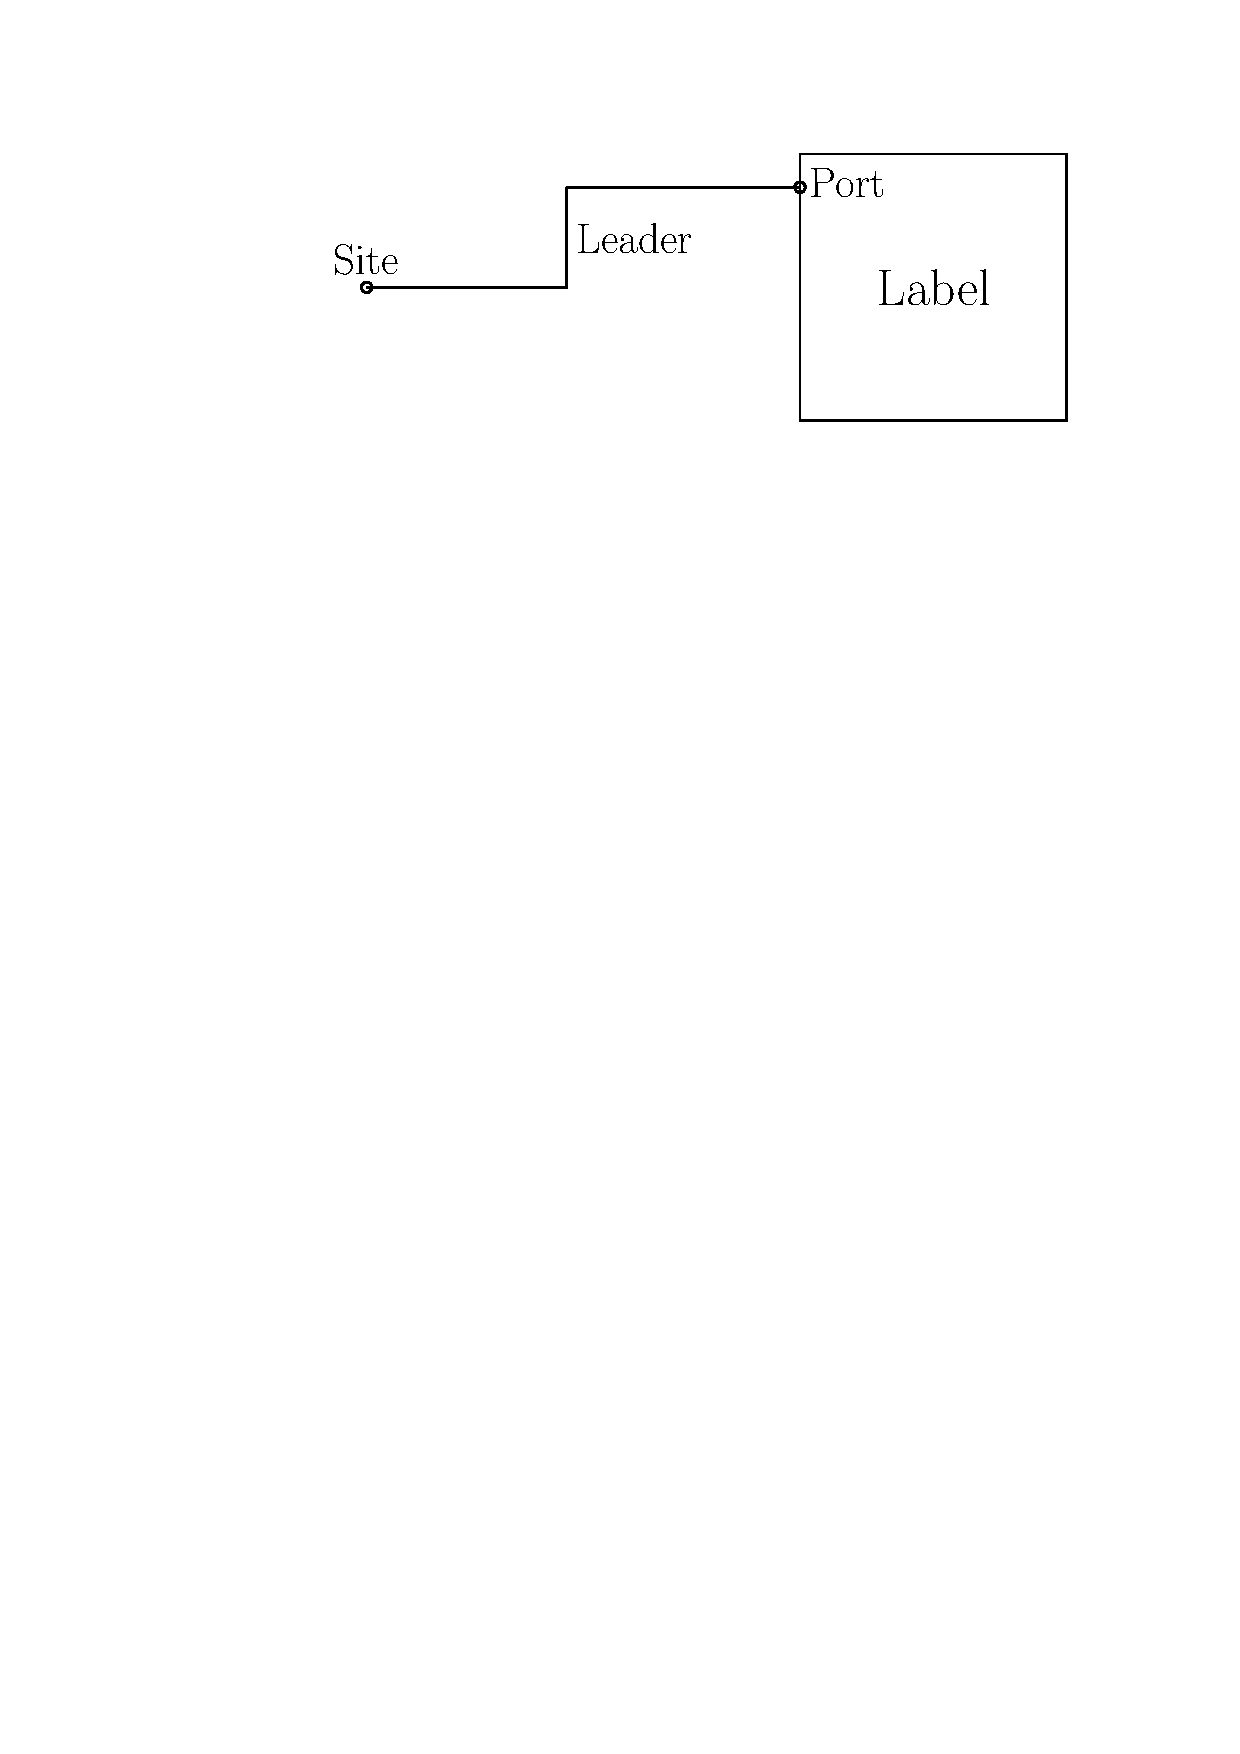
\includegraphics[scale=0.5]{IPE_TerminologyDrawing.pdf}
  \caption{Illustrated guide to the labeling terminology}
 \label{fig:term}
\end{figure}

\begin{itemize}
 \item \textbf{Graph:} A Set of Vertices and Edges (see below), often used to represent routing problems. Can be further classified depending on its properties.
 \item \textbf{Edge:} A connection between two vertices, usually represented as a line. Can be directional, limiting its usage, or have a cost (``Weight'') associated with its use.
 \item \textbf{Vertex:} A featureless object that can be connected to any number other vertices via edges. Usually depicted as a point or small shape. Commonly also referred to as \textbf{``Node''}, as will be the the case in this paper.
 \item \textbf{Label:} Additional information, usually represented as a box containing the additional information. Will also be referred to as \textbf{``Annotation''} in this paper.
 \item \textbf{Site:} The point, object or word that is labeled - without it, there wouldn't be any labeling necessary.
 \item \textbf{Leader:} The path connecting the site to the label - depending on its shape, it can be described further using several subgroups which can be freely combined to form new leader types:
  \begin{itemize}
   \item \textit{S-Leader:} This Leader connects site and label in a straight line.
   \item \textit{O-Leader:} This leader runs orthogonally to the border between text and label area.
   \item \textit{P-Leader:} This Leader runs parallel to the border between text and label area. It must be combined with other leader styles, as it won't reach the label area otherwise.
  \end{itemize}
    For example, the leader from Fig.~\ref{fig:term} would be classified as an opo-Leader.
 \item \textbf{Port:} The location where the leader connects to the label. It may be restricted pre-determined locations, like only at the corners.
  \item \textbf{Monotonous/Monotonicity:} Describes a steady progression towards a direction or goal. Will be used in this paper to indicate that there's no loss of progress made from the site to the label, effectively restricting the direction a leader can go at each bend.
\end{itemize}
%Mehr Graphenterminologie? (zb: Path) +Polylinien Vertex/Node für Knoten in Polylinien bzw. Graphen -->Eindeutig!

\section{The program}

In our program, the focus was put on keeping the text as readable as possible. This means that leaders are only allowed in the space between words or lines, which can make certain locations for sites unavailable, as there might already too many leaders routed through that area to insert yet another for the new site. 
We also wanted the leaders to be monotonous, which means that they will be one of the shortest possible connection between port and site locations.
Our final priority was to efficiently use the space for the labels, which meant that each label should initially be placed as close to the available area's border as possible.
While this allows for more space in which labels can be placed, it also means that the distance between Label and site often increases, which leads to longer leaders.%''Final Priority'' klingt komisch -> Ersatz finden!

%Algorithmus(Ansatz) und Implementierung(noch immer abstrakt) trennen! Probleme, Details, ... gegen Ende!
\subsection{Algorithm}%''Underlying Algorithm''?
To easily create paths that exclusively use the space between words and lines, we decided to use a graph similar to the one Loose \cite{Loose2015} used, placing nodes above and below each word's beginning and end, and connecting them with their horizontally and vertically adjacent neighbours.%Umformulieren?
For the sites, we inserted an additional node above the center of the word, which will serve as the leader's starting point. We also decided to give the graph's edges a capacity of 1, which means that each leader will always use edges which haven't already be taken by other leaders. While this causes some sites to become un-routable due to another leader passing right through their starting node, it makes visualizing the leaders much easier. Our first approach was going through the labels in the order they appear in the text and placing each as far up as possible, to maximize the remaining space other labels could use.

Since putting the labels right next to the text would result in the labels' positions being restricted by the text's line spacing,we decided to leave a buffer zone in between the two areas, which allows the leaders to adjust between the position forced by the line spacing and the label's final position. As this allowed us to place the labels more freely, we adjusted the label's positions after all labels were placed to reduce the distance that needed to be covered in the buffer area.

\subsection{Implementation}
The program was written in Java, using only JGraphT\cite{JGraphT} as additional library. Since we only want to create leaders that don't intersect with the text, the graph was created alongside the placement of the words on the canvas, as it was easy to extract measurements at this point. Due to some problems with Java's various methods of calculating linebreaks, this process was done completely by hand. Since the Graph's nodes represent fixed locations on the canvas, they each have coordinates associated with them, with the nodes representing the sites containing extra information, such as references to the corresponding annotation and to the leader connecting the two (if existent).
%TODO: Code genauer durchlesen und erweitern!


%Similar to Loose's Approach\cite{Loose2015}, we used a Graph to model the available routing space for the algorithm. As a result of this approach, it is important to know exactly where each word is placed. While Java offers a function that automatically places text in lines of given width, it does so in a way that doesn't allow the content of each line to be read as a String afterwards, which makes it unusable for our purposes. Therefore each word must be placed manually, and to since it isn't the main focus of the program, each series of characters between a space is considered one word that has to be fully placed within one line.

%Using the dimensions of each word, we create the graph by creating and connecting nodes in the space between lines at the start and end of each word, and at the end of the text area. We also create special nodes for each annotated word, they are located above the word in a central position. Each node also is located at set co-ordinates, which allows the routing algorithms to easily fulfill the monotonicity constraint.
%We left some space in between the text area and the label area %Name=?(Lass dir was einfallen)
%to allow the labels to be placed more freely. While the routing graph only reaches up to the border of the text area, the connection between the graph and the label is done with an OPO-Leader. As there is the possibility of intersecting with other leaders, this means some extra adjustments have to be done. For demonstration purposes, we also included another algorithm that uses S-Leaders for this section.

%(Potential) Problems/Issues, solutions



%Section Ideas: The Program/Framework (Modellerklärung), The Algorithm(s), Implementation, Evaluation, Conclusion


\bibliographystyle{plain}
\bibliography{references}

\end{document}